%%%%%%%%%%%%%%%%%%%%%%%%%%%%%%%%%%%%%%%%%%%%%%%%%%%%%%%%%%%%%%%%%%%%%%
% LaTeX Example: Project Report
%
% Source: http://www.howtotex.com
%
% Feel free to distribute this example, but please keep the referral
% to howtotex.com
% Date: March 2011 
% 
%%%%%%%%%%%%%%%%%%%%%%%%%%%%%%%%%%%%%%%%%%%%%%%%%%%%%%%%%%%%%%%%%%%%%%
% How to use writeLaTeX: 
%
% You edit the source code here on the left, and the preview on the
% right shows you the result within a few seconds.
%
% Bookmark this page and share the URL with your co-authors. They can
% edit at the same time!
%
% You can upload figures, bibliographies, custom classes and
% styles using the files menu.
%
% If you're new to LaTeX, the wikibook is a great place to start:
% http://en.wikibooks.org/wiki/LaTeX
%
%%%%%%%%%%%%%%%%%%%%%%%%%%%%%%%%%%%%%%%%%%%%%%%%%%%%%%%%%%%%%%%%%%%%%%
% Edit the title below to update the display in My Documents
%\title{Project Report}
%
%%% Preamble
\documentclass[paper=letter, fontsize=10pt]{scrartcl}
\usepackage[T1]{fontenc}
\usepackage{fourier}

\usepackage[english]{babel}															% English language/hyphenation
\usepackage[protrusion=true,expansion=true]{microtype}	
\usepackage{amsmath,amsfonts,amsthm} % Math packages
\usepackage[pdftex]{graphicx}	
\usepackage{url}
\usepackage{enumerate}
\usepackage{lastpage}
\usepackage{float}


%%% Custom sectioning
\usepackage{sectsty}
\allsectionsfont{\normalfont\scshape}


%%% Custom headers/footers (fancyhdr package)
\usepackage{fancyhdr}
\pagestyle{fancy}
\fancyhead[L]{}
\fancyhead[c]{Design Revision 0 Revision 0}
\fancyhead[R]{\today}											
\fancyfoot[L]{}											 
\fancyfoot[C]{}											
\fancyfoot[R]{\thepage\ of \pageref{LastPage}}		% Pagenumbering
\renewcommand{\headrulewidth}{0.4pt}				% Remove header underlines
\renewcommand{\footrulewidth}{0.4pt}				% Remove footer underlines
\setlength{\headheight}{13.6pt}


%%% Equation and float numbering
\numberwithin{equation}{section}		% Equationnumbering: section.eq#
\numberwithin{figure}{section}			% Figurenumbering: section.fig#
\numberwithin{table}{section}				% Tablenumbering: section.tab#


%%% Maketitle metadata
\newcommand{\horrule}[1]{\rule{\linewidth}{#1}} 	% Horizontal rule
\newcommand{\ts}{\textsuperscript}

%%% Begin document
\begin{document}

\begin{titlepage}

\newcommand{\HRule}{\rule{\linewidth}{0.5mm}} % Defines a new command for the horizontal lines, change thickness here
\newcommand{\authors}{\shortstack{Vitaliy Kondratiev,\\Nathan Johrendt,\\Tyler Lyn,\\Mark Gammie}}

\begin{center}
 
%----------------------------------------------------------------------------------------
%	HEADING SECTIONS
%----------------------------------------------------------------------------------------

\textsc{\LARGE McMaster University}\\[1.5cm] % Name of your university/college
\textsc{\Large CAS 4ZP6}\\[0.5cm]
\textsc{\Large Team 9} \\[0.5cm]
\textsc{\Large Capstone Project 2013/2014}\\[0.5cm] % Major heading such as course name
\textsc{\large Porter Simulation}\\[0.5cm] % Minor heading such as course title

%----------------------------------------------------------------------------------------
%	TITLE SECTION
%----------------------------------------------------------------------------------------

\HRule \\[0.4cm]
{ \huge \bfseries Design Revision 0}\\[0.4cm] % Title of your document
\HRule \\[1.5cm]
 
%----------------------------------------------------------------------------------------
%	AUTHOR SECTION
%----------------------------------------------------------------------------------------

\begin{minipage}{0.4\textwidth}
\begin{flushleft} \large
\emph{Authors:}\\
Vitaliy Kondratiev\\
Nathan Johrendt\\
Tyler Lyn\\
Mark Gammie
\end{flushleft}
\end{minipage}
~
\begin{minipage}{0.4\textwidth}
\begin{flushright} \large
\emph{Supervisor:} \\
Dr. Douglas Down % Supervisor's Name
\end{flushright}
\end{minipage}\\[4cm]

% If you don't want a supervisor, uncomment the two lines below and remove the section above
%\Large \emph{Author:}\\
%John \textsc{Smith}\\[3cm] % Your name

%----------------------------------------------------------------------------------------
%	DATE SECTION
%----------------------------------------------------------------------------------------

{\large \today}\\[3cm] % Date, change the \today to a set date if you want to be precise

%----------------------------------------------------------------------------------------
%	LOGO SECTION
%----------------------------------------------------------------------------------------

%\includegraphics{Logo}\\[1cm] % Include a department/university logo - this will require the graphicx package
 
%----------------------------------------------------------------------------------------
%Template taken from: http://www.softwaretestinghelp.com/test-plan-sample-softwaretesting-and-quality-assurance-templates/

\vfill % Fill the rest of the page with whitespace
\end{center}
\end{titlepage}

\setcounter{tocdepth}{2}

\tableofcontents

\newpage

\section{Revision History}
\begin{center}
    \begin{tabular}{| c | l | l | l |}
    \hline
    Revision \# & Author & Date & Comment \\ \hline
  	1 & \shortstack{\\Vitaliy Kondratiev,\\Nathan Johrendt,\\Tyler Lyn,\\Mark Gammie} & January 11, 2014 & Revision 0 Added to repository \\ \hline
    \end{tabular}
\end{center}

\section{Executive Summary}
\subsection{Introduction}
\subsection{Purpose}
\subsection{Design Overview}
\section{Implementation Material}
\subsection{Language of Implementation}
\subsection{Supporting Technology and Frameworks}
\newpage
\subsection{Process Diagram}
\begin{figure}[H]
	\begin{center}
		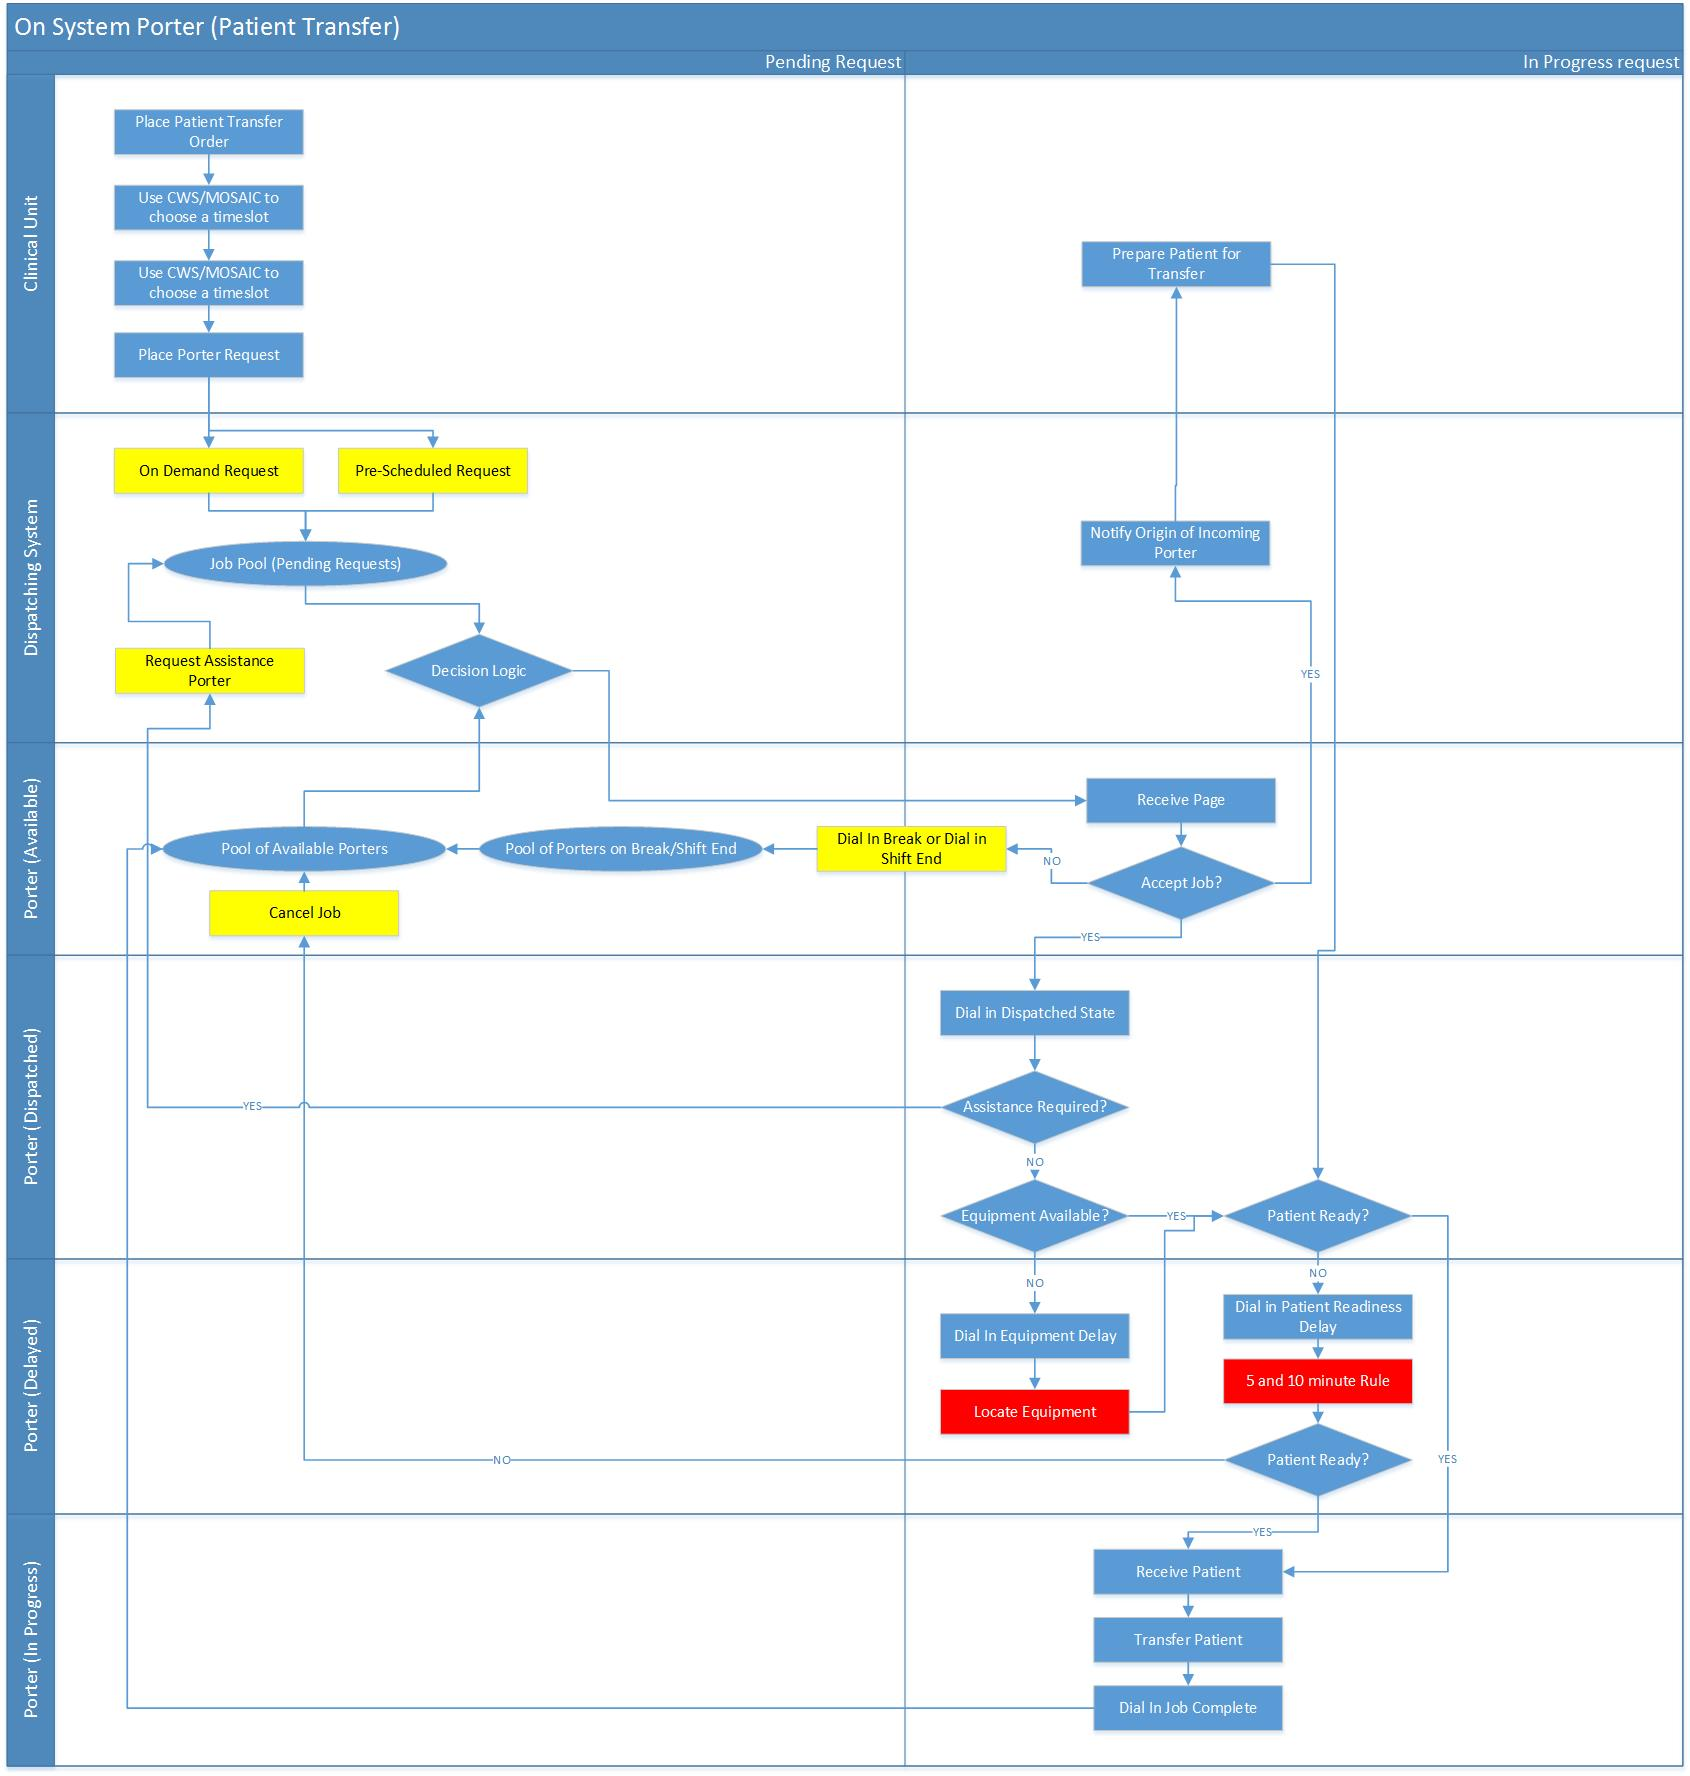
\includegraphics[width=1\columnwidth]{../Process Diagrams/Process Diagram.jpg}
		\caption{Process Diagram}
	\end{center}
\end{figure}
\newpage
\section{Dependency Diagram}

\begin{figure}[H]
	\begin{center}
		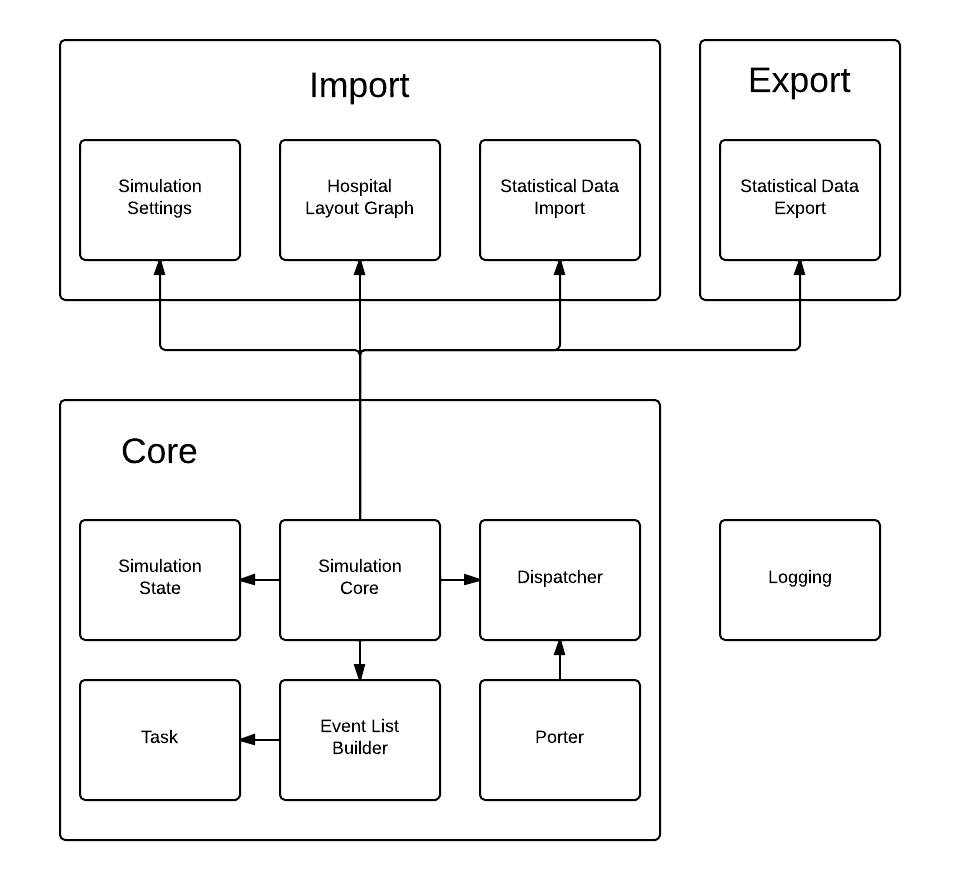
\includegraphics[width=1\columnwidth]{../Process Diagrams/Dependency Diagram.png}
		\caption{Dependency Diagram}
	\end{center}
\end{figure}
\newpage

\section{Decomposition Description}
\subsection{Core - Simulation Core}
\begin{enumerate}[]
	\item \textbf{Type:} Module
	\item \textbf{Purpose:} 
	\item \textbf{Function:} 
	\item \textbf{Interface:}
	\item \textbf{Process Steps:} 
	\item \textbf{Data:}
	\item \textbf{Error Handling:}
	\item \textbf{Requirement Reference:}
	\item \textbf{Critical Revision 0 Component:} True
\end{enumerate}
\subsection{Core - Simulation State}
\begin{enumerate}[]
	\item \textbf{Type:} Module
	\item \textbf{Purpose:} 
	\item \textbf{Function:} 
	\item \textbf{Interface:}
	\item \textbf{Process Steps:} 
	\item \textbf{Data:}
	\item \textbf{Error Handling:}
	\item \textbf{Requirement Reference:}
	\item \textbf{Critical Revision 0 Component:} True
\end{enumerate}
\subsection{Core - Task}
\begin{enumerate}[]
	\item \textbf{Type:} Module
	\item \textbf{Purpose:} 
	\item \textbf{Function:} 
	\item \textbf{Interface:}
	\item \textbf{Process Steps:} 
	\item \textbf{Data:}
	\item \textbf{Error Handling:}
	\item \textbf{Requirement Reference:}
	\item \textbf{Critical Revision 0 Component:} True
\end{enumerate}
\subsection{Core - Event List Builder}
\begin{enumerate}[]
	\item \textbf{Type:} Module
	\item \textbf{Purpose:} 
	\item \textbf{Function:} 
	\item \textbf{Interface:}
	\item \textbf{Process Steps:} 
	\item \textbf{Data:}
	\item \textbf{Error Handling:}
	\item \textbf{Requirement Reference:}
	\item \textbf{Critical Revision 0 Component:} True
\end{enumerate}
\subsection{Core - Porter}
\begin{enumerate}[]
	\item \textbf{Type:} Module
	\item \textbf{Purpose:} 
	\item \textbf{Function:} 
	\item \textbf{Interface:}
	\item \textbf{Process Steps:} 
	\item \textbf{Data:}
	\item \textbf{Error Handling:}
	\item \textbf{Requirement Reference:}
	\item \textbf{Critical Revision 0 Component:} True
\end{enumerate}
\subsection{Core - Dispatcher}
\begin{enumerate}[]
	\item \textbf{Type:} Module
	\item \textbf{Purpose:} 
	\item \textbf{Function:} 
	\item \textbf{Interface:}
	\item \textbf{Process Steps:} 
	\item \textbf{Data:}
	\item \textbf{Error Handling:}
	\item \textbf{Requirement Reference:}
	\item \textbf{Critical Revision 0 Component:} True
\end{enumerate}
\subsection{Import - Simulation Setting}
\begin{enumerate}[]
	\item \textbf{Type:} Module
	\item \textbf{Purpose:} 
	\item \textbf{Function:} 
	\item \textbf{Interface:}
	\item \textbf{Process Steps:} 
	\item \textbf{Data:}
	\item \textbf{Error Handling:}
	\item \textbf{Requirement Reference:}
	\item \textbf{Critical Revision 0 Component:} True
\end{enumerate}
\subsection{Import - Hospital Layout Graph}
\begin{enumerate}[]
	\item \textbf{Type:} Module
	\item \textbf{Purpose:} 
	\item \textbf{Function:} 
	\item \textbf{Interface:}
	\item \textbf{Process Steps:} 
	\item \textbf{Data:}
	\item \textbf{Error Handling:}
	\item \textbf{Requirement Reference:}
	\item \textbf{Critical Revision 0 Component:} True
\end{enumerate}
\subsection{Import - Statistical Data Import}
\begin{enumerate}[]
	\item \textbf{Type:} Module
	\item \textbf{Purpose:} 
	\item \textbf{Function:} 
	\item \textbf{Interface:}
	\item \textbf{Process Steps:} 
	\item \textbf{Data:}
	\item \textbf{Error Handling:}
	\item \textbf{Requirement Reference:}
	\item \textbf{Critical Revision 0 Component:} True
\end{enumerate}
\subsection{Export - Statistical Data Export}
\begin{enumerate}[]
	\item \textbf{Type:} Module
	\item \textbf{Purpose:} 
	\item \textbf{Function:} 
	\item \textbf{Interface:}
	\item \textbf{Process Steps:} 
	\item \textbf{Data:}
	\item \textbf{Error Handling:}
	\item \textbf{Requirement Reference:}
	\item \textbf{Critical Revision 0 Component:} True
\end{enumerate}
\subsection{Logging}
\begin{enumerate}[]
	\item \textbf{Type:} Module
	\item \textbf{Purpose:} 
	\item \textbf{Function:} 
	\item \textbf{Interface:}
	\item \textbf{Process Steps:} 
	\item \textbf{Data:}
	\item \textbf{Error Handling:}
	\item \textbf{Requirement Reference:}
	\item \textbf{Critical Revision 0 Component:} True
\end{enumerate}
\section{Anticipated Changes}
\begin{enumerate}[1]
	\item Change 1
\end{enumerate}

%%% End document
\end{document}